\documentclass[11pt]{article}

% Packages
\usepackage{microtype}
\usepackage[english]{babel}
\usepackage{fontspec}
\usepackage[cm]{fullpage}
\usepackage{titlesec}
\usepackage{titling}
\usepackage[backend=biber,style=musuos]{biblatex}
\usepackage{hyperref}     
\usepackage{graphicx}     
\usepackage{caption}
\usepackage[top=1cm,left=2cm,right=2cm,bottom=2cm]{geometry}

% Settings
\newfontfamily\headingfont[]{Neris Light}
\setmainfont{Gelasio Regular}
\setsansfont{Neris Light}
\setmonofont{Fira Code}

\renewcommand{\maketitlehooka}{\normalfont\headingfont\Huge\bfseries}
\titleformat{\section}
{\normalfont\headingfont\LARGE\bfseries}
{\thesection}{1em}{}
\titleformat{\subsection}
{\normalfont\headingfont\large\bfseries}
{\thesection}{1em}{}

\addbibresource{desinc.bib}

% Metadata
\title{Graphical authoring of interactive applications with i-score}
\author{Jean-Michaël Celerier\\ \small Blue Yeti\thanks{\url{http://www.blueyeti.fr}}, SCRIME\thanks{\url{http://scrime.labri.fr}}, LaBRI\thanks{\url{http://www.labri.fr}}}
\date{}

% https://desinc.mfm.sussex.ac.uk/#cfp 
\begin{document}
\maketitle
\vspace{-3cm}	
\section*{Presentation}
The following workshop aims to present the use of the i-score (\url{www.i-score.org}) temporal interaction design software.

The workshop will first present the challenges and the rationale that led to the creation of the software, that is, the lack of dedicated tools for precise temporal design.

Then, the construction of a score will be detailed on practical examples involving audio and video features and interaction with a familiar creative coding environment.

\begin{figure}[h]
	\centering
	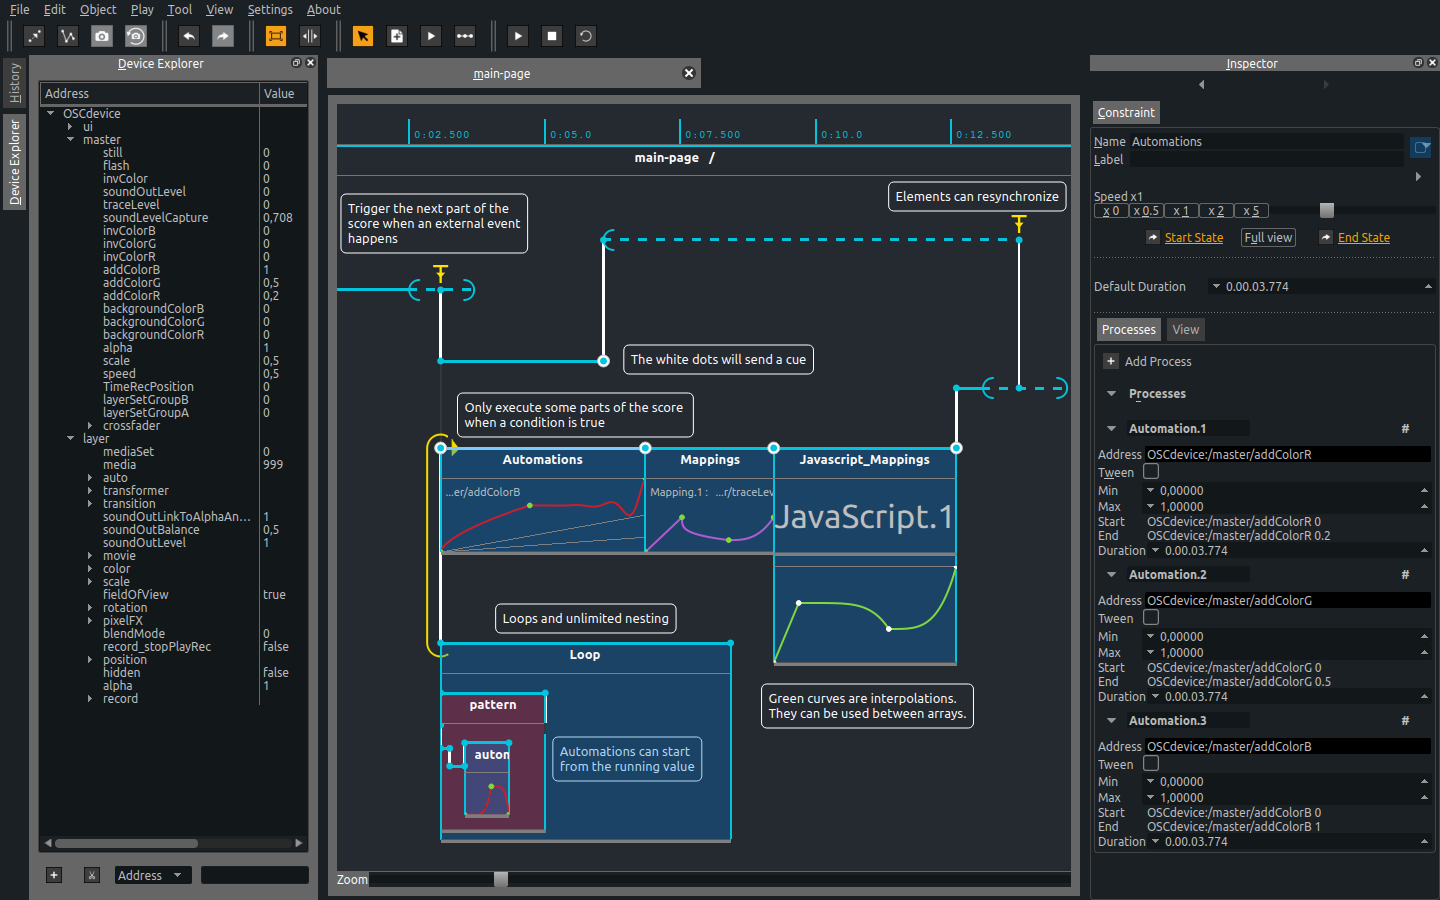
\includegraphics[width=0.5\textwidth]{images/iscore.png}
	\caption*{A score in the i-score software}
\end{figure}One of the core goals of this project is to make most features accessible without resorting to programming. This is meant to maximize usability by designers who may not have a computer science background, as often required with other creative environments.

\subsection*{Workshop objectives}
The main objective is for the participants to be able to use the i-score software autonomously by the end of the workshop.

This means:

\begin{itemize}
	\item Comprehension of the temporal elements offered by the software paradigm, usage of the different parts of the user interface.
	\item Authoring of both linear (score-like) and non-linear (installation-like) programs.
	\item Orchestration of common multimedia software with i-score: PureData, Max/MSP, Unity3D, Processing, and more generally any kind of OSC-compliant software.
	Some of these software are able to use the Minuit protocol via extensions\footnote{\url{http://www.jamoma.org} and \url{https://github.com/OSSIA/}} which allows for a tight integration between the actual media application, and i-score.
	\item Leveraging the temporal features of i-score to handle common problematic cases in the case of interactive installations:~applications with multiple states such as interactive user interface with several pages, and error or exceptional case handling.
	\item Leveraging the i-score JavaScript API for problems easily solved by a code snippet, such as complex arithmetic computations or deeply-intertwined conditions.
	\item An overview of the incorporated audio features that allow to create interactive musical scores without the need to resort to an external software.
\end{itemize}

\section*{Requirements}
\subsection*{Requirements for participants}
There is no formal requirement, but it would be better for the
participants to have familiarity with at least one creative coding environment,
such as Max/MSP, PureData, OpenFrameworks, Processing.

The software in itself is free software, available for Linux, Mac, and Windows computers from the website.
Text tutorials and documentation are also provided as a reference.\subsection*{Technical requirements}
For a better experience, the participants should have a Mac computer with Max/MSP to be able to follow the workshop steps on their own. The workshop is also opened to OpenFrameworks or Processing users, although the latest versions of these environments do not provide a deep integration with i-score.

\section*{Presenter biography}
Jean-Michaël Celerier\footnote{\url{http://jcelerier.name/}}, born 1992, is a ph.~d. student in computer science and multimedia interaction, under an industrial agreement between the company Blue Yeti and the Université de Bordeaux, where he is part of the SCRIME~(Research \& Creation Studio in Computer Science and Experimental Music).

He did an engineering cursus in computer science and multimedia technologies, and aims to decrease the barrier of entry to interactive music making with his work. His personal interests include music recording, guitar playing, and creative coding.

\nocite{baltazar_i-score_2014}
\nocite{de2016presentation}
\nocite{celerier2015ossia}
\nocite{celerier2016outils}

\printbibliography
\end{document}